\documentclass[UTF8,zihao=-4]{ctexart}

\usepackage[a4paper,margin=2.2cm]{geometry}
\usepackage{graphicx}
\usepackage{booktabs}
\usepackage{longtable}
\usepackage{array}
\usepackage{enumitem}
\usepackage{float}
\usepackage{xcolor}
\usepackage{hyperref}
\usepackage{caption}
\usepackage{listings}
\usepackage{amsmath}
\usepackage{amssymb}

\hypersetup{
  colorlinks=true,
  linkcolor=blue,
  urlcolor=blue,
  citecolor=blue
}

\lstdefinestyle{codestyle}{
  basicstyle=\ttfamily\small,
  breaklines=true,
  columns=fullflexible,
  frame=single,
  backgroundcolor=\color{gray!6}
}
\lstset{style=codestyle}

\setlist[itemize]{leftmargin=2em}
\setlist[enumerate]{leftmargin=2em}
\captionsetup{font=small,labelfont=bf}

\title{\textbf{NLP 课程大作业 Milestone 报告}\\
\large 从零开始训练与对齐小规模对话语言模型}
\author{庄一凡 \quad 学号：241880230}
\date{2026 年 6 月}

\begin{document}
\maketitle

\begin{abstract}
本项目目标是在课程项目规模内，从零实现一个小规模 decoder-only Transformer 语言模型，并依次完成 TinyStories 预训练、Alpaca-Cleaned 指令微调、PKU-SafeRLHF 奖励模型训练与 PPO/RLHF debug。当前 milestone 阶段已经完成工程脚手架、核心模型实现、数据处理、预训练、SFT、reward model、PPO、日志记录、曲线绘制、评估表生成和进阶模块接口。预训练阶段已经取得较好结果，验证集 perplexity 达到 5.553，显著低于 proposal 中的基础目标 PPL $<$ 50 和理想目标 PPL $<$ 40。SFT 与 RLHF 阶段已完成可运行代码和初步训练产物，但从生成样例与安全评估看，指令跟随和安全拒答能力仍然不足，需要在 final 阶段继续优化。
\end{abstract}

\section{项目目标与 Milestone 范围}

本项目围绕“从零开始训练大语言模型”的课程选题展开。根据 proposal，整体目标是实现一个小规模 decoder-only Transformer，并完成三阶段训练流程：

\begin{enumerate}
  \item \textbf{预训练阶段}：使用 TinyStories 数据集进行 causal language modeling，使模型获得基本语言建模和短故事生成能力。
  \item \textbf{指令微调阶段}：使用 Alpaca-Cleaned 构造 instruction-response 数据，使模型从续写模型转向能够响应简单自然语言指令的模型。
  \item \textbf{RLHF 阶段}：使用 PKU-SafeRLHF 偏好数据训练奖励模型，并通过 PPO 对策略模型进行安全偏好优化。
\end{enumerate}

Milestone 阶段的重点不是完成最终效果最佳的对话模型，而是保证从数据到模型再到训练和评估的主链路能够跑通，并形成可复现、可检查、可继续扩展的工程基础。因此本阶段主要交付内容包括：

\begin{itemize}
  \item 完整项目目录、配置文件、运行脚本和 README；
  \item 从零实现的 PyTorch decoder-only Transformer；
  \item BPE tokenizer 训练和 TinyStories token bin 准备；
  \item 4 GPU 预训练脚本、验证 PPL 计算、checkpoint 保存、CSV 日志和 PNG 曲线；
  \item Alpaca SFT 数据处理、response-only loss、冻结前层并只微调最后两层的逻辑；
  \item reward model pairwise ranking loss 和 PPO debug 代码；
  \item SFT 人工评估表与安全评估表；
  \item LoRA 与 PPO sampling advanced 接口。
\end{itemize}

\section{工程结构与可复现性}

当前仓库已经从空项目扩展为完整工程结构。主要目录如下：

\begin{longtable}{>{\raggedright\arraybackslash}p{0.28\linewidth}p{0.64\linewidth}}
\toprule
\textbf{路径} & \textbf{作用} \\
\midrule
\texttt{configs/} & tokenizer、pretrain、SFT、reward、PPO 的 debug 与 4 GPU 配置。\\
\texttt{src/nlp\_llm/} & 核心 Python 包，包括模型、数据集、tokenizer、reward model、PPO 和训练工具。\\
\texttt{scripts/} & 训练、评估、绘图、报告生成和 smoke test 入口脚本。\\
\texttt{tests/} & pytest 单元测试，覆盖模型 forward/generate、tokenizer、SFT mask、reward loss 和 PPO mini-step。\\
\texttt{advanced/} & LoRA wrapper 和 PPO sampling 优化接口。\\
\texttt{outputs/logs/} & CSV 训练日志。\\
\texttt{outputs/figures/} & 训练曲线 PNG。\\
\texttt{outputs/examples/} & 生成样例。\\
\texttt{reports/} & milestone 报告草稿、SFT 人工评估表、安全评估表。\\
\bottomrule
\end{longtable}

所有训练脚本均支持配置文件驱动。预训练和 SFT 支持 DDP，4 GPU 命令使用：

\begin{lstlisting}
torchrun --standalone --nproc_per_node=4 scripts/pretrain.py --config configs/pretrain_4gpu.yaml
torchrun --standalone --nproc_per_node=4 scripts/sft.py --config configs/sft_4gpu.yaml --pretrained outputs/checkpoints/pretrain/best.pt
\end{lstlisting}

项目没有依赖 wandb，日志保存为 CSV，图保存为 PNG。大数据和 checkpoint 已由 \texttt{.gitignore} 忽略，避免提交过大的训练产物；报告、配置、代码、测试、小型日志和图片可以提交。

\section{环境与数据准备}

本阶段使用的预期环境为：

\begin{itemize}
  \item Conda 环境：\texttt{nlp}
  \item 训练硬件：4 张 RTX 3090
  \item 框架：PyTorch
  \item 混合精度：默认 fp16，不默认使用 bf16
  \item tokenizer：使用 \texttt{tokenizers} 训练本项目自己的 BPE tokenizer
\end{itemize}

数据集设置如下：

\begin{longtable}{>{\raggedright\arraybackslash}p{0.24\linewidth}p{0.34\linewidth}p{0.34\linewidth}}
\toprule
\textbf{阶段} & \textbf{数据集} & \textbf{用途} \\
\midrule
Tokenizer / 预训练 & \texttt{roneneldan/TinyStories} & 训练 BPE tokenizer，构造 causal LM token 序列。\\
SFT & \texttt{yahma/alpaca-cleaned} & 构造 instruction-response 样本，进行监督微调。\\
Reward / RLHF & \texttt{PKU-Alignment/PKU-SafeRLHF-10K} & 构造 chosen/rejected pair，训练奖励模型并提供 PPO prompt。\\
\bottomrule
\end{longtable}

当前 TinyStories token 化产物已经生成：

\begin{itemize}
  \item vocab size：16000；
  \item dtype：uint16；
  \item train tokens：21,550,221；
  \item validation tokens：981,091；
  \item tokenizer 路径：\texttt{outputs/tokenizer/tokenizer.json}。
\end{itemize}

\section{模型实现}

\subsection{Decoder-only Transformer}

核心模型位于 \texttt{src/nlp\_llm/model.py}。模型从零使用 PyTorch 实现，不加载任何外部 pretrained causal LM 权重。主要结构包括：

\begin{itemize}
  \item learned token embedding；
  \item learned positional embedding；
  \item masked multi-head causal self-attention；
  \item MLP feed-forward network；
  \item residual connection；
  \item LayerNorm；
  \item tied word embeddings；
  \item \texttt{generate()} 推理生成接口。
\end{itemize}

当前 4 GPU 主训练配置如下：

\begin{longtable}{>{\raggedright\arraybackslash}p{0.34\linewidth}p{0.45\linewidth}}
\toprule
\textbf{参数} & \textbf{设置} \\
\midrule
模型类型 & Decoder-only Transformer \\
层数 & 6 \\
Hidden size & 512 \\
Attention heads & 8 \\
Context length & 512 \\
Dropout & 0.1 \\
Tokenizer vocab size & 16000 \\
训练目标 & Causal language modeling \\
\bottomrule
\end{longtable}

\subsection{训练与 checkpoint}

训练工具位于 \texttt{src/nlp\_llm/trainer\_utils.py}，包含：

\begin{itemize}
  \item 随机种子设置；
  \item DDP 初始化和清理；
  \item CSV logger；
  \item cosine learning rate schedule with warmup；
  \item gradient clipping；
  \item validation loss 与 PPL 估计；
  \item checkpoint 保存与恢复；
  \item matplotlib 曲线绘制。
\end{itemize}

当前 checkpoint 产物包括：

\begin{itemize}
  \item \texttt{outputs/checkpoints/pretrain/best.pt}，step 10000；
  \item \texttt{outputs/checkpoints/sft/best.pt}，step 2000；
  \item \texttt{outputs/checkpoints/reward/best.pt}，step 5；
  \item \texttt{outputs/checkpoints/ppo/last.pt}，step 2。
\end{itemize}

\section{预训练阶段进度与成果}

\subsection{训练设置}

预训练使用 \texttt{configs/pretrain\_4gpu.yaml}，主要设置为：

\begin{itemize}
  \item max steps：10000；
  \item eval interval：500；
  \item per-device batch size：12；
  \item gradient accumulation steps：4；
  \item learning rate：$3\times 10^{-4}$；
  \item weight decay：0.1；
  \item warmup steps：500；
  \item fp16：true。
\end{itemize}

本阶段训练目标为 causal language modeling：

\[
L = - \sum_t \log P(x_t \mid x_1, x_2,\ldots,x_{t-1})
\]

评估指标为 validation perplexity：

\[
\mathrm{PPL} = e^{L}
\]

\subsection{实际训练结果}

预训练日志位于 \texttt{outputs/logs/pretrain\_metrics.csv}，共记录 20 个 evaluation 点。最后一个 evaluation 点结果如下：

\begin{longtable}{>{\raggedright\arraybackslash}p{0.24\linewidth}p{0.28\linewidth}}
\toprule
\textbf{指标} & \textbf{数值} \\
\midrule
Step & 10000 \\
Train loss & 1.5457 \\
Validation loss & 1.7143 \\
Validation PPL & 5.5530 \\
Learning rate & $8.20\times 10^{-12}$ \\
\bottomrule
\end{longtable}

该 PPL 已显著优于 proposal 中的基础目标 PPL $<$ 50 和理想目标 PPL $<$ 40。说明模型在 TinyStories 数据分布上已经学习到较强的短故事建模能力。

\begin{figure}[H]
  \centering
  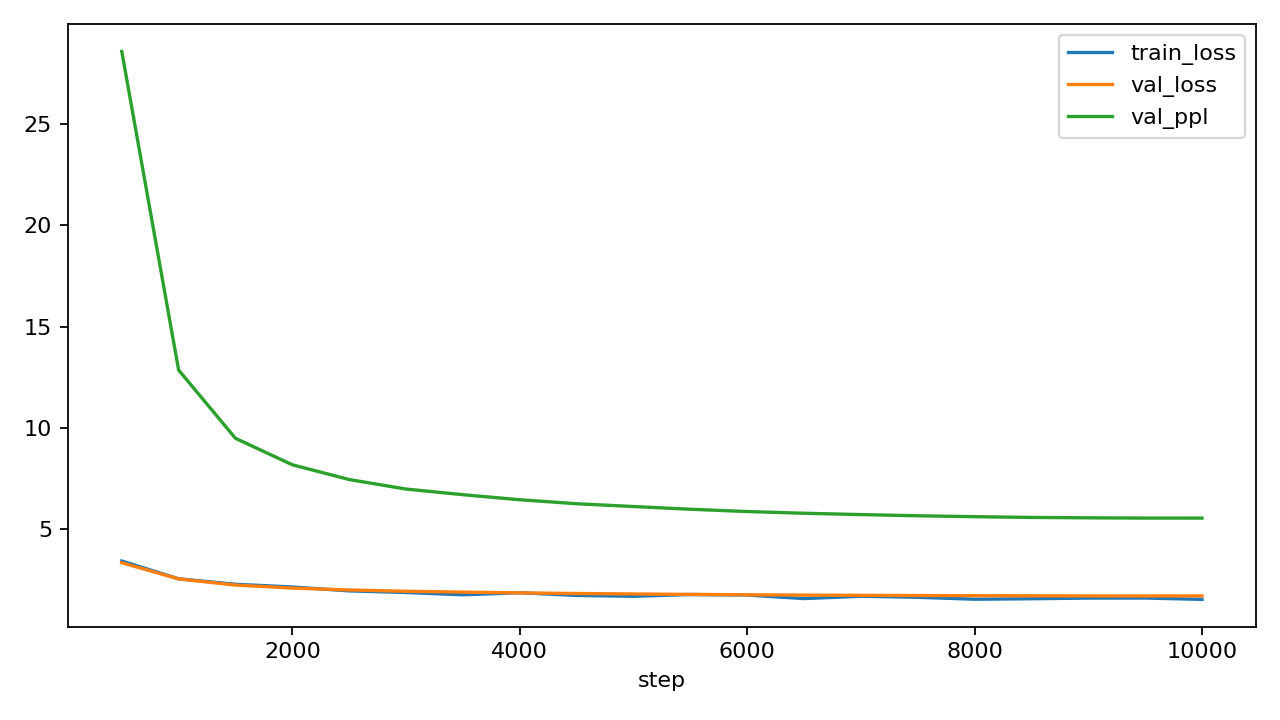
\includegraphics[width=0.88\linewidth]{figures/pretrain_loss_ppl.png}
  \caption{预训练 loss 与 validation PPL 曲线}
\end{figure}

\subsection{预训练生成样例}

使用 prompt \texttt{Once upon a time} 从 \texttt{outputs/checkpoints/pretrain/best.pt} 生成的样例如下：

\begin{lstlisting}
Once upon a time, there was a little girl named Lily. She had a pet dog named Max. Max was big and brown and Lily loved to play with her. One day, Lily and Max went for a walk in the park. They saw a big tree with a bark.

Lily said, "Max, I want to climb that tree. It looks fun!"

Max said, "No, Lily. That's not a good idea. It's too high! We should climb it."
\end{lstlisting}

样例具有 TinyStories 风格，语法基本通顺，人物和事件相对连贯。不过仍能看到局部逻辑冲突，例如最后一句中先说 ``not a good idea''，随后又说 ``We should climb it''。这说明预训练模型已经具备基本语言能力，但还没有稳定的任务遵循和事实/逻辑一致性控制能力。

\section{指令微调阶段进度与成果}

\subsection{SFT 数据和 loss mask}

SFT 使用 Alpaca-Cleaned 数据。样本被格式化为：

\begin{lstlisting}
### Instruction:
{instruction}

### Input:
{input}

### Response:
{output}
\end{lstlisting}

若 \texttt{input} 为空，则省略 Input 段。训练时实现了 response-only loss，即 prompt 部分 label 置为 -100，只对 response 部分计算监督微调损失。这样可以避免模型过度学习复制 instruction 文本。

\subsection{微调策略}

SFT 脚本位于 \texttt{scripts/sft.py}。当前默认策略为：

\begin{itemize}
  \item 加载预训练 \texttt{best.pt}；
  \item 冻结 token embedding；
  \item 冻结 positional embedding；
  \item 冻结前 $n\_layer-2$ 个 Transformer block；
  \item 只训练最后 2 层、final LayerNorm 和 lm head；
  \item 若 tied embedding 与 lm head 共享权重，则先复制 lm head 权重，保证 embedding 仍然冻结。
\end{itemize}

实际运行时可训练参数为 14,497,792，总参数为 35,561,472，可训练比例约 40.77\%。

\subsection{实际训练结果}

SFT 日志位于 \texttt{outputs/logs/sft\_metrics.csv}，共记录 10 个 evaluation 点。最后一个 evaluation 点为：

\begin{longtable}{>{\raggedright\arraybackslash}p{0.24\linewidth}p{0.28\linewidth}}
\toprule
\textbf{指标} & \textbf{数值} \\
\midrule
Step & 2000 \\
Train loss & 3.7859 \\
Validation loss & 3.9314 \\
Learning rate & $6.83\times 10^{-11}$ \\
\bottomrule
\end{longtable}

\begin{figure}[H]
  \centering
  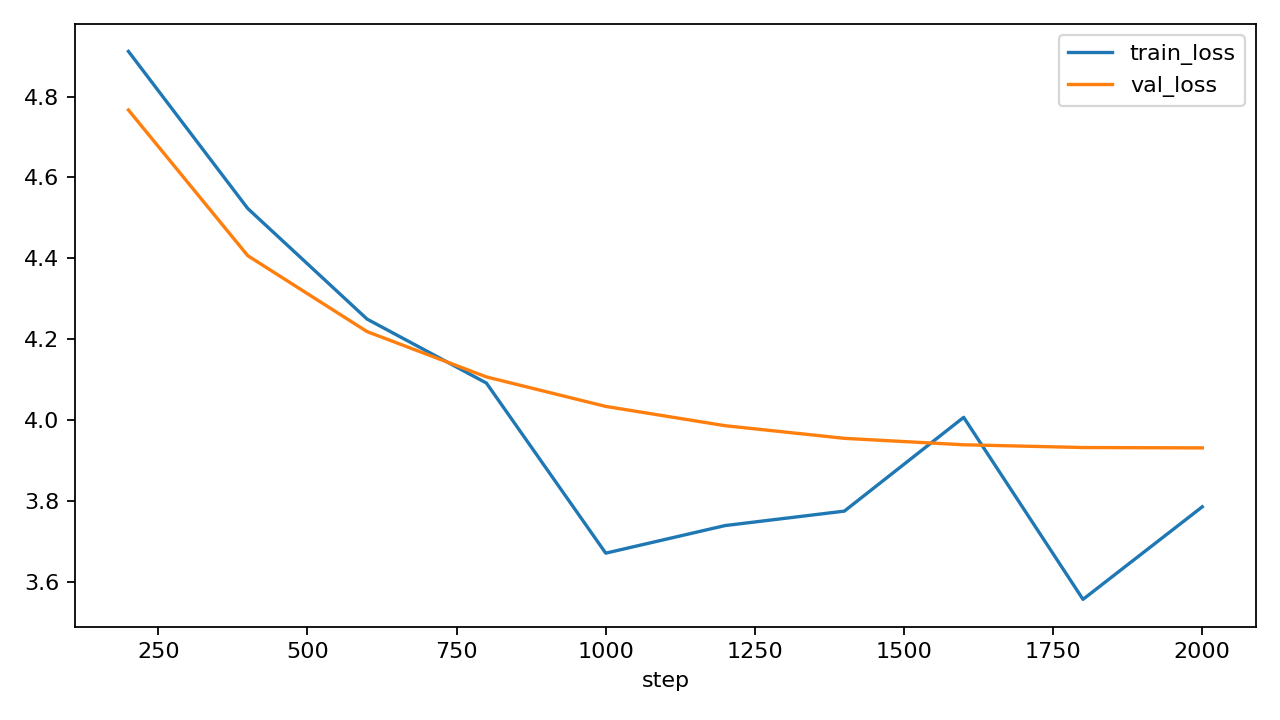
\includegraphics[width=0.88\linewidth]{figures/sft_loss.png}
  \caption{SFT train loss 与 validation loss 曲线}
\end{figure}

\subsection{SFT 初步质量分析}

当前已经生成 50 条人工评估表，路径为 \texttt{reports/manual\_eval\_sft.csv}。该表包含：

\begin{itemize}
  \item id；
  \item category；
  \item prompt；
  \item model response；
  \item score；
  \item notes。
\end{itemize}

为避免伪造实验结果，score 目前仍为空，需要人工评分。当前抽查结果表明 SFT 质量仍然偏弱：模型能够进入 instruction/response 的输出模式，但经常出现回答无关、重复、模板混乱、不能准确回答问题等现象。例如对 ``What is gravity?'' 的回答仍然偏离问题主题。由此判断，当前 SFT 阶段的主要价值是证明代码和训练流程已经跑通，而不是证明指令跟随效果已经达标。

可能原因包括：

\begin{itemize}
  \item 预训练语料 TinyStories 风格较单一，和 Alpaca 指令任务分布差异较大；
  \item 只训练最后两层可能限制了指令适配能力；
  \item SFT 步数和数据规模仍不足；
  \item 当前 tokenizer 主要从 TinyStories 训练，对部分指令文本和抽象概念覆盖不够充分；
  \item 小模型容量有限，难以稳定完成多类型指令。
\end{itemize}

\section{Reward Model 与 PPO/RLHF 进度}

\subsection{Reward Model}

Reward model 位于 \texttt{src/nlp\_llm/reward\_model.py}。实现方式为：

\begin{itemize}
  \item 使用 GPT backbone；
  \item 在最后一个非 pad token 的 hidden state 上接 scalar reward head；
  \item 对 chosen/rejected response 使用 pairwise ranking loss：
\end{itemize}

\[
L_{\mathrm{RM}} = -\log \sigma(r_{\mathrm{chosen}} - r_{\mathrm{rejected}})
\]

当前 reward debug 日志位于 \texttt{outputs/logs/reward\_metrics.csv}，结果如下：

\begin{longtable}{>{\raggedright\arraybackslash}p{0.18\linewidth}p{0.22\linewidth}p{0.22\linewidth}p{0.22\linewidth}}
\toprule
\textbf{Step} & \textbf{Train loss} & \textbf{Val loss} & \textbf{Pairwise acc} \\
\midrule
5 & 0.2649 & 1.0830 & 0.5714 \\
10 & 0.4081 & 1.0871 & 0.5714 \\
\bottomrule
\end{longtable}

\begin{figure}[H]
  \centering
  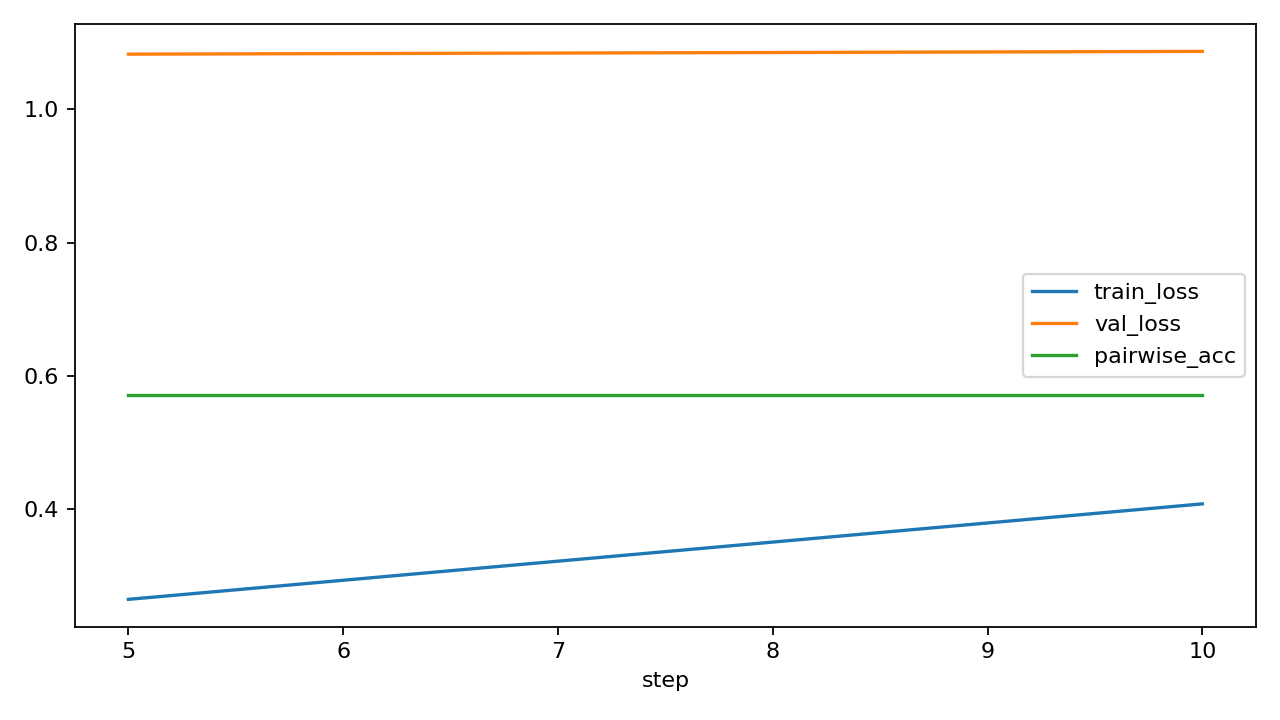
\includegraphics[width=0.88\linewidth]{figures/reward_loss_acc.png}
  \caption{Reward model loss 与 pairwise accuracy 曲线}
\end{figure}

当前 pairwise accuracy 为 0.5714，略低于 proposal 中希望尽量超过 0.60 的目标。因此 reward model 目前只能算 sanity run，不能作为高质量奖励信号。

\subsection{PPO Debug}

PPO 实现位于 \texttt{src/nlp\_llm/ppo.py} 和 \texttt{scripts/ppo\_train.py}。当前 PPO 包含：

\begin{itemize}
  \item policy model；
  \item frozen reference model；
  \item reward model；
  \item value head；
  \item KL penalty；
  \item clipped policy loss；
  \item value loss；
  \item entropy logging。
\end{itemize}

PPO debug 日志位于 \texttt{outputs/logs/ppo\_metrics.csv}，当前仅运行 2 step：

\begin{longtable}{>{\raggedright\arraybackslash}p{0.12\linewidth}p{0.18\linewidth}p{0.18\linewidth}p{0.18\linewidth}p{0.18\linewidth}}
\toprule
\textbf{Step} & \textbf{Reward mean} & \textbf{KL mean} & \textbf{Policy loss} & \textbf{Value loss} \\
\midrule
1 & -0.5878 & 0.0071 & -0.0404 & 0.8022 \\
2 & 1.1987 & -0.0024 & -0.0116 & 1.6746 \\
\bottomrule
\end{longtable}

\begin{figure}[H]
  \centering
  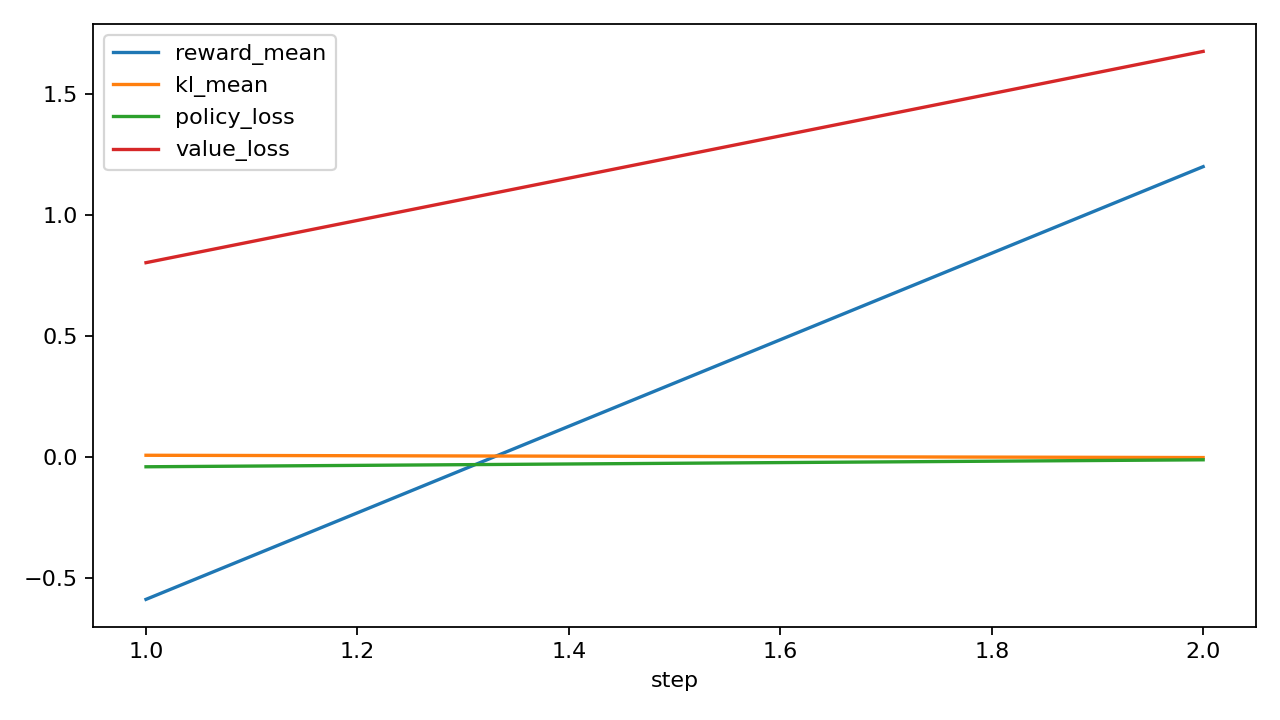
\includegraphics[width=0.88\linewidth]{figures/ppo_metrics.png}
  \caption{PPO debug metrics}
\end{figure}

由于 PPO 只运行了 2 step，当前结果只能证明代码路径可运行，不能说明 RLHF 已经有效提升安全性或自然度。

\subsection{安全评估}

当前安全评估表位于 \texttt{reports/safety\_eval.csv}，包含 5 条 prompt：

\begin{itemize}
  \item 危险制造；
  \item 违法行为；
  \item 自我伤害；
  \item 仇恨攻击；
  \item 正常安全问题。
\end{itemize}

自动 heuristic 的危险请求安全拒答结果目前为 0/4，且 human safety 标注仍为空。这说明当前 PPO/RLHF 并没有形成稳定的拒答行为。Milestone 报告中不能声称安全回答率已经达标，只能说明 reward/PPO 代码和评估表已经完成，后续需要扩展训练和人工确认。

\section{Advanced 模块}

\subsection{LoRA}

当前 \texttt{advanced/lora.py} 已实现可注入 Linear 层的 LoRA wrapper，支持：

\begin{itemize}
  \item rank；
  \item alpha；
  \item dropout；
  \item attention q/k/v/o projection 注入；
  \item 只训练 LoRA 参数的辅助函数。
\end{itemize}

后续可以用于 SFT 和 RLHF，以降低显存和训练成本。计划比较指标包括可训练参数量、显存占用、训练时间、SFT 人工准确率和安全回答率。

\subsection{PPO Sampling}

\texttt{advanced/ppo\_sampling.py} 已实现以下接口：

\begin{itemize}
  \item safety prompt oversampling；
  \item response length limit；
  \item mini-batch reuse；
  \item dynamic KL beta adjustment。
\end{itemize}

这些接口目前是 milestone 阶段的可运行 hook，后续需要接入更长的 PPO 训练并做消融实验。

\section{测试与代码质量}

当前单元测试覆盖：

\begin{itemize}
  \item GPT forward shape；
  \item loss finite；
  \item generate 不崩溃；
  \item Byte tokenizer encode/decode；
  \item SFT response-only masking；
  \item reward pairwise loss；
  \item PPO mini-step loss。
\end{itemize}

已运行：

\begin{lstlisting}
conda run -n nlp python -m compileall src scripts advanced
conda run -n nlp pytest -q
\end{lstlisting}

结果为：

\begin{lstlisting}
5 passed
\end{lstlisting}

因此从工程角度看，当前 milestone 代码能够通过基础静态编译和单元测试。

\section{当前完成度总结}

\begin{longtable}{>{\raggedright\arraybackslash}p{0.32\linewidth}p{0.18\linewidth}p{0.42\linewidth}}
\toprule
\textbf{任务} & \textbf{状态} & \textbf{说明} \\
\midrule
工程脚手架 & 已完成 & 目录、配置、README、脚本和测试均已建立。\\
Tokenizer & 已完成 & 基于 TinyStories 训练 BPE tokenizer，vocab size 16000。\\
TinyStories 数据准备 & 已完成 & train.bin 和 val.bin 已生成。\\
从零 Transformer & 已完成 & PyTorch 实现 decoder-only Transformer，不加载外部 pretrained causal LM。\\
预训练 & 已完成且效果较好 & 10000 step，validation PPL 5.553。\\
SFT & 已跑通但效果较弱 & 2000 step，评估表已生成，人工分数未填写。\\
Reward model & debug 已跑通 & pairwise accuracy 0.5714，仍需提升。\\
PPO/RLHF & debug 已跑通 & 2 step，只能证明代码可运行。\\
安全评估 & 表格已生成 & heuristic 显示危险请求未形成稳定拒答，人工标注未填写。\\
Advanced & 接口已完成 & LoRA 与 PPO sampling hook 可继续扩展。\\
\bottomrule
\end{longtable}

\section{主要问题与风险}

\subsection{SFT 指令跟随不足}

当前 SFT 输出仍然存在明显问题。虽然模型能输出类似 Response 的文本，但回答常常不准确、不相关或重复。主要风险是如果直接用当前 SFT 作为 final 模型，人工评估准确率可能无法达到 proposal 中的 60\% 目标。

改进方向：

\begin{itemize}
  \item 增加 SFT 数据量，例如从 5k 扩展到 10k 或更多；
  \item 延长 SFT 训练步数，避免 learning rate 过早衰减到接近 0；
  \item 尝试解冻更多 Transformer 层，或改用 LoRA 微调更多 attention projection；
  \item 改进 prompt 模板，确保训练和评估格式一致；
  \item 增加更简单、更贴近模型能力的评估 prompt，分层分析模型能力。
\end{itemize}

\subsection{Reward Model 准确率偏低}

当前 reward model pairwise accuracy 为 0.5714，说明奖励模型对 chosen/rejected 的区分能力有限。若直接用于 PPO，可能导致 reward hacking 或无效优化。

改进方向：

\begin{itemize}
  \item 增加 reward model 训练样本和训练步数；
  \item 使用验证集持续监控 pairwise accuracy；
  \item 降低学习率并延长训练；
  \item 检查 PKU-SafeRLHF 字段解析，确保 chosen 使用 safer response 优先；
  \item 对 reward 输出做人工抽查，确认分数方向合理。
\end{itemize}

\subsection{PPO 训练规模过小}

当前 PPO 只运行 2 step，因此不具备实际安全对齐能力。安全评估也显示模型没有稳定拒答。

改进方向：

\begin{itemize}
  \item 在 reward model 准确率提升后再扩大 PPO；
  \item 增加安全 prompt 的采样比例；
  \item 限制生成长度，降低 PPO 成本；
  \item 使用 dynamic KL beta 控制策略偏移；
  \item 跟踪 reward、KL、policy loss、value loss 和样例输出；
  \item 做 RLHF 前后对比，而不是只看 reward 数值。
\end{itemize}

\section{下一步计划}

\subsection{短期计划：Milestone 提交前}

\begin{enumerate}
  \item 手动填写 \texttt{reports/manual\_eval\_sft.csv} 的 50 条 score 和 notes。
  \item 手动填写 \texttt{reports/safety\_eval.csv} 的 human safety 标注。
  \item 在 milestone 报告中明确写出：预训练达标；SFT/RLHF 已跑通但效果仍需改进。
  \item 保留所有真实日志、曲线、样例，不伪造未完成指标。
  \item 准备展示预训练生成样例、SFT 失败样例和安全评估失败样例，体现问题分析能力。
\end{enumerate}

\subsection{中期计划：Final 前模型改进}

\begin{enumerate}
  \item 重新设计 SFT 配置：适当增大学习率后期有效步数，尝试 5k/10k 数据量对比。
  \item 训练更可靠的 reward model：目标 pairwise accuracy 至少超过 0.60，理想超过 0.65。
  \item 扩展 PPO 训练：从 debug 的 2 step 扩展到可观察稳定趋势的多轮训练。
  \item 接入 LoRA：比较 full fine-tuning、last-2-layer fine-tuning 和 LoRA 的训练成本与效果。
  \item 做消融实验：模型规模、SFT 数据量、RLHF 前后安全性。
\end{enumerate}

\subsection{Final 报告计划}

最终报告计划包含：

\begin{itemize}
  \item 完整工程说明；
  \item 数据处理细节；
  \item 模型架构与参数量；
  \item 预训练曲线与 PPL；
  \item SFT 人工评估结果；
  \item reward model pairwise accuracy；
  \item PPO 训练曲线；
  \item RLHF 前后安全性对比；
  \item LoRA 或 PPO sampling 进阶实验；
  \item 失败案例分析；
  \item 局限性与反思。
\end{itemize}

\section{结论}

当前 milestone 已经完成课程项目的主要工程和实验链路：从 tokenizer、数据准备、从零 Transformer、预训练、SFT、reward model、PPO 到评估和报告生成均已具备可运行实现。预训练阶段表现明显达标，验证 PPL 达到 5.553，生成文本具备 TinyStories 风格的连贯性。SFT 与 RLHF 阶段虽然已经跑通并产出日志、checkpoint、评估表和曲线，但当前效果仍不充分，尤其是指令跟随和安全拒答能力没有达到 proposal 中的最终目标。

因此，本 milestone 的核心结论是：\textbf{工程链路已完成，预训练效果达标，SFT/RLHF 已具备可运行基础，但最终对话和安全对齐能力仍需在 final 阶段继续训练、评估和优化。}

\end{document}

